% This is samplepaper.tex, a sample chapter demonstrating the
% LLNCS macro package for Springer Computer Science proceedings;
% Version 2.21 of 2022/01/12
%
\documentclass{llncs}
%
\usepackage[T1]{fontenc}
% T1 fonts will be used to generate the final print and online PDFs,
% so please use T1 fonts in your manuscript whenever possible.
% Other font encondings may result in incorrect characters.
%
\usepackage{graphicx}
% Used for displaying a sample figure. If possible, figure files should
% be included in EPS format.
%
% If you use the hyperref package, please uncomment the following two lines
% to display URLs in blue roman font according to Springer's eBook style:
%\usepackage{color}
%\renewcommand\UrlFont{\color{blue}\rmfamily}
%\urlstyle{rm}
%

\usepackage[style=apa]{biblatex} % <- AGREGAR ESTA LÍNEA
\addbibresource{Referencias.bib} % <- AGREGAR ESTA LÍNEA

\renewcommand{\tablename}{Tabla}

\hyphenation{e-va-luar}
\hyphenation{con-si-de-rar}
\hyphenation{mo-de-lo}
\hyphenation{va-ria-bles}


\begin{document}
%
% ENGLISH VERSION
\title{Analysis of cardiological data with machine learning tools}

%\titlerunning{Abbreviated paper title}
% If the paper title is too long for the running head, you can set
% an abbreviated paper title here
%
\author{Nicolás Seivane\inst{1}\orcidID{0000-1111-2222-3333} \and
Andrea Rey\inst{1}\orcidID{0000-0002-9185-1382}}
%
\authorrunning{N. Seivane et al.}
% First names are abbreviated in the running head.
% If there are more than two authors, 'et al.' is used.
%
\institute{
Laboratorio de Investigación y Desarrollo Experimental en Computación (LIDEC),
 Universidad Nacional de Hurlingham (UNAHUR), Buenos Aires, Argentina
\email{seivanenicolas@gmail.com, andrea.rey@unahur.edu.ar}}
%
\maketitle              % typeset the header of the contribution
%
\begin{abstract}
In the current landscape where medical practices, such as cardiology, generate an unprecedented volume of data whose complexity often exceeds the capabilities of conventional analysis, machine learning tools emerge as a resource capable of extracting phenotypic patterns hidden within clinical datasets, thereby obtaining additional information for a holistic view of the patient's cardiovascular status. 
%This methodology should not only be seen as a technological innovation, but as a fundamental analytical tool applied to cardiological data, making it possible to identify digital biomarkers and disease trajectories that were previously imperceptible, thus laying the groundwork for a more efficient and personalized clinical practice.
In the present work, a comparative analysis of machine learning techniques applied to cardiological data is conducted. Classical algorithms were implemented and evaluated, including Naïve Bayes, Logistic Regression, Random Forest, and Support Vector Machines. The study includes predictive models for heart failure and fetal cardiotocography. The results indicate that the best overall performing method is Random Forest, achieving a high generalization capacity in both scenarios.
In this context, the implementation of advanced computational models could be used to design preventive strategies based on algorithmic evidence and the analysis of historical data. It is important to highlight that machine learning does not aim to replace clinical judgment, but rather to strengthen it, functioning as a support tool for the interpretation of diagnostic tests, optimizing response times in critical cardiac intensive care environments.

% keywords in lowercase
\keywords{Cardiology\and Machine Learning\and Classification}
\end{abstract}

% SPANISH VERSION
% Clear the previous title info and set Spanish version

% Spanish title and abstract
\begin{center}
\vspace{1cm}
{\Large \bfseries\boldmath Análisis de datos cardiológicos con herramientas de aprendizaje automático}

\vspace{0.5cm}
\end{center}

\begin{abstract}

En el escenario actual donde prácticas médicas, como  cardiología, generan un volumen de datos sin precedentes, cuya complejidad a menudo excede las capacidades del análisis convencional, las herramientas de aprendizaje automático emergen como un recurso capaz de extraer patrones fenotípicos ocultos en conjuntos de datos clínicos, obteniendo así información adicional para una visión holística del estado cardiovascular del paciente.
% Esta metodología no solo debe verse como una innovación tecnológica, sino como una herramienta analítica fundamental aplicada a datos cardiológicos, siendo posible identificar biomarcadores digitales y trayectorias de enfermedad que antes resultaban imperceptibles, sentando así las bases para una práctica clínica más eficiente y personalizada. 
En el presente trabajo se realiza un análisis comparativo de técnicas de aprendizaje automático aplicadas a datos cardiológicos. Se implementaron y evaluaron algoritmos clásicos, como Naïve Bayes, Regresión Logística, \emph{Random Forest} y Máquinas de Vectores de Soporte. El estudio incluye modelos de predicción para insuficiencia cardíaca y para cardiotocografía fetal. Los resultados indican que el método con mejor desempeño general es \emph{Random Forest}, logrando una alta capacidad de generalización en ambos escenarios. 
En este contexto, la implementación de modelos computacionales avanzados podría utilizarse para diseñar estrategias preventivas basadas en la evidencia algorítmica y el análisis de datos históricos. Es importante resaltar que el aprendizaje automático no pretende sustituir el juicio clínico, sino fortalecerlo, funcionando como una herramienta de soporte para la interpretación de pruebas diagnósticas, optimizando los tiempos de respuesta en entornos críticos de cuidados intensivos cardiológicos.


% palabras clave en minúsculas
\keywords{Cardiología\and Aprendizaje Automático\and Clasificación}
\end{abstract}


\vspace{0.5cm}
\setcounter{page}{1}

%
\section{Introducción}

Las enfermedades cardiovasculares representan la principal causa de muerte a nivel mundial, cobrando aproximadamente $17,9$ millones de vidas al año, lo que equivale al $31\%$ de las defunciones globales. El proceso de diagnóstico tradicional, aunque efectivo, puede ser extenso y depende del análisis de parámetros clínicos estructurados, señales cardíacas como el electrocardiograma (ECG) e imágenes médicas. Herramientas como el ECG, las pruebas de esfuerzo y los ecocardiogramas son el estándar clínico actual, pero requieren una interpretación obligatoria experta que puede beneficiarse de la agilidad de los modelos computacionales de Aprendizaje Automático (AA).
El objetivo central de este estudio es evaluar el rendimiento de técnicas de AA al realizar predicciones sobre la posible presencia de insuficiencia cardíaca. Se exploran no solo casos de clasificación binaria (enfermo/sano), sino también el caso multiclase para el estudio de la cardiotocografía (CTG), que evalúa el bienestar fetal. Basándose en el estado del arte~\parencite{isaksen2025evaluating,kumar2021machine}, que destaca el uso de modelos como Máquinas de Vectores de Soporte (SVM, por sus siglas en inglés)~\parencite{Cortes1995} y Naïve Bayes (NB)~\parencite{hand2001idiot}, para la detección de arritmias y cardiopatías, este trabajo busca validar estas técnicas en un entorno comparativo con conjuntos de datos reales, bajo métricas de calidad estándar.
Diversos estudios han demostrado una efectividad moderada, por lo que se requiere del escrutinio médico sobre los resultados obtenidos al aplicar algoritmos de AA y métodos de ensamble en problemas de clasificación médica. En particular, \emph{Random Forest} (RF, por sus siglas en inglés)~\parencite{breiman2017classification}, ha mostrado un alto desempeño debido a su capacidad para modelar relaciones no lineales y reducir el sobreajuste mediante la combinación de múltiples árboles de decisión. Asimismo, técnicas de interpretabilidad de la explicabilidad de variables (también llamadas características o atributos), como la importancia por permutación, permiten identificar aquellas variables más influyentes, contribuyendo a la comprensión del modelo, siendo éstas las más importantes para el modelo y no en el estudio, el cual debe estar determinado y diseñado por un experto del área de salud.


\section{Materiales y métodos}

En este trabajo se utilizaron dos conjuntos de datos: por un lado, \emph{HeartFailure}~\parencite{HeartFailure}, compuesto por 918 registros con dos posibles etiquetas, correspondientes a un problema de clasificación binaria, y por otro lado, \emph{Cardiotocography}~\parencite{Cardiotocografia}, con 2115 registros, incluyendo las clases `normal', `sospechoso' y `patológico', representando así a un problema de clasificación multiclase. Ambos conjuntos  contienen variables clínicas relevantes utilizadas para el análisis y predicción de condiciones cardiovasculares, como por ejemplo, la presión sanguínea, el nivel de colesterol en sangre, la presencia de dolor de pecho, la frecuencia cardíaca, entre otras.
Para cada uno de estos conjuntos, se realizó un proceso de preparación incluyendo análisis exploratorio, verificación de la ausencia de valores faltantes, validación de la consistencia de tipos de datos y codificación de variables categóricas cuando fue necesario. Este proceso permitió asegurar la calidad de los datos antes del entrenamiento de los modelos.

Se implementaron cuatro algoritmos de clasificación: Regresión Logística (RL)~\parencite{cramer2002origins}, SVM, NB Gaussiano, y RF. Cada modelo requiere de la optimización de  hiperparámetros (valores que debe fijar el usuario antes de construir los modelos) que influyen en su capacidad de generalización y en el equilibrio entre sesgo y varianza, incluyendo la compensación entre un posible sobreajuste (\emph{overfitting}) o un posible subajuste (\emph{underfitting}).
%RL fue optimizado mediante el ajuste del parámetro de regularización, el tipo de penalización y el algoritmo de optimización, lo que permite controlar el sobreajuste y mejorar la convergencia. En el modelo SVM, se optimizaron el parámetro de regularización, el tipo de kernel y el coeficiente, que determinan la forma de la frontera de decisión. En el caso de NB Gaussiano, se ajustó el parámetro de suavizado, que permite mejorar la estabilidad numérica y evitar problemas derivados de varianzas cercanas a cero. Finalmente, para RF, se ajustaron el criterio de partición, la profundidad máxima de los árboles y la cantidad de variables consideradas en cada división de los nodos, parámetros que afectan la complejidad del modelo y su capacidad de capturar relaciones no lineales.	
La optimización de hiperparámetros se realizó mediante búsqueda en grilla combinada con validación cruzada $k$-\emph{folds}, con $k=5$, lo que permite evaluar el modelo en múltiples particiones del conjunto de datos y obtener estimaciones sólidas de su desempeño.
Para la evaluación de los clasificadores, se utilizaron métricas estándar de clasificación, incluyendo \emph{accuracy}, que mide la proporción de registros correctamente clasificados; F1-\emph{Score}, definido como la media armónica entre la calidad de predicción de la clase positiva y la capacidad de detección, y Área Bajo la Curva ROC (AUC por sus siglas en inglés). Además, se aplicó el método de importancia por permutación~\parencite{breiman2017classification}, que consiste en medir la disminución del desempeño del modelo al alterar aleatoriamente cada variable, permitiendo estimar su contribución relativa.	

\section{Resultados y discusión}

Luego de optimizar los hiperparámetros, se obtuvo la mejor configuración para SVM con kernel radial en el caso binario y polinómico de grado $2$ en el caso multiclase, con coeficiente igual a $0,1$ y a $1$ en los casos binario y multiclase, respectivamente, y costo de violación de restricción igual a $1$ y a $0,1$ al considerar dos o tres clases, respectivamente. El modelo RF se optimizó utilizando el criterio de la entropía para el caso binario y con el criterio de Gini en el caso multiclase, con una profundidad máxima de $7$ en el caso binario y sin restricción para el caso multiclase, y $5$ o $2$ muestras como mínimo en cada partición para los casos binario y multiclase, respectivamente. En el caso de NB, los diferentes valores de suavizado no introdujeron modificaciones en el rendimiento del modelo.
%Los resultados obtenidos en la Tabla~\ref{tab:métricas} para el caso binario (izquierda) y para el caso multiclase (derecha), muestran que el modelo RF presentó el mejor desempeño en ambos conjuntos de datos, seguido por SVM y RL. Esto confirma la capacidad de los métodos de AA para capturar relaciones complejas en los datos clínicos.
Los resultados de la Tabla~\ref{tab:métricas} para el caso binario (izq.) y para el caso multiclase (der.) muestran que RF tuvo el mejor desempeño en ambos casos, alcanzando los valores más altos de \emph{accuracy} ($0,8782$ y $0,9432$), F1-\emph{Score} ($0,8775$ y $0,9412$) y AUC ($0,9315$ y $0,9868$), tanto en el caso binario como en el multiclase. El modelo SVM con kernel radial también mostró un desempeño competitivo, especialmente en el caso binario, mientras que RL presentó resultados sólidos en el problema multiclase, aunque con menor capacidad para capturar relaciones no lineales complejas. 
%Estos resultados confirman la efectividad de los modelos basados en múltiples árboles de decisión para el análisis de datos clínicos.

\begin{table}
\centering
\caption{Métricas de evaluación en los casos binario (izq.) y multiclase (der.). }\label{tab:métricas}
\begin{tabular}{|l|r|r|r|cc|l|r|r|r|}
\cline{1-4}  \cline{7-10}
\textbf{Modelo}	& \textbf{\emph{Accuracy}} &	\textbf{F1-\emph{Score}} & \textbf{AUC} & & & \textbf{Modelo}	& \textbf{\emph{Accuracy}} &	\textbf{F1-\emph{Score}} & \textbf{AUC} \\ 
\cline{1-4}  \cline{7-10}
RL &	$0,8485$ &	$0,8481$ & $0,9050$ & & & RL &	$0,8485$	& $0,8481$	& $0,9050$ \\
SVM & 	$0,8616$ &	$0,8609$ &	$0,9232$ & & & SVM	& $0,8616$ &	$0,8609$ &	$0,9232$ \\
NB	& $0,8420$	& $0,8420$ &	$0,9138$ & & & NB	& $0,8420$	& $0,8420$	& $0,9138$ \\
RF	& $0,8780$	& $0,8775$ &	$0,9315$ & & & RF	& $0,8780$	& $0,8775$	& $0,9315$
\\
\cline{1-4}  \cline{7-10}
\end{tabular}
\end{table}

\begin{figure}
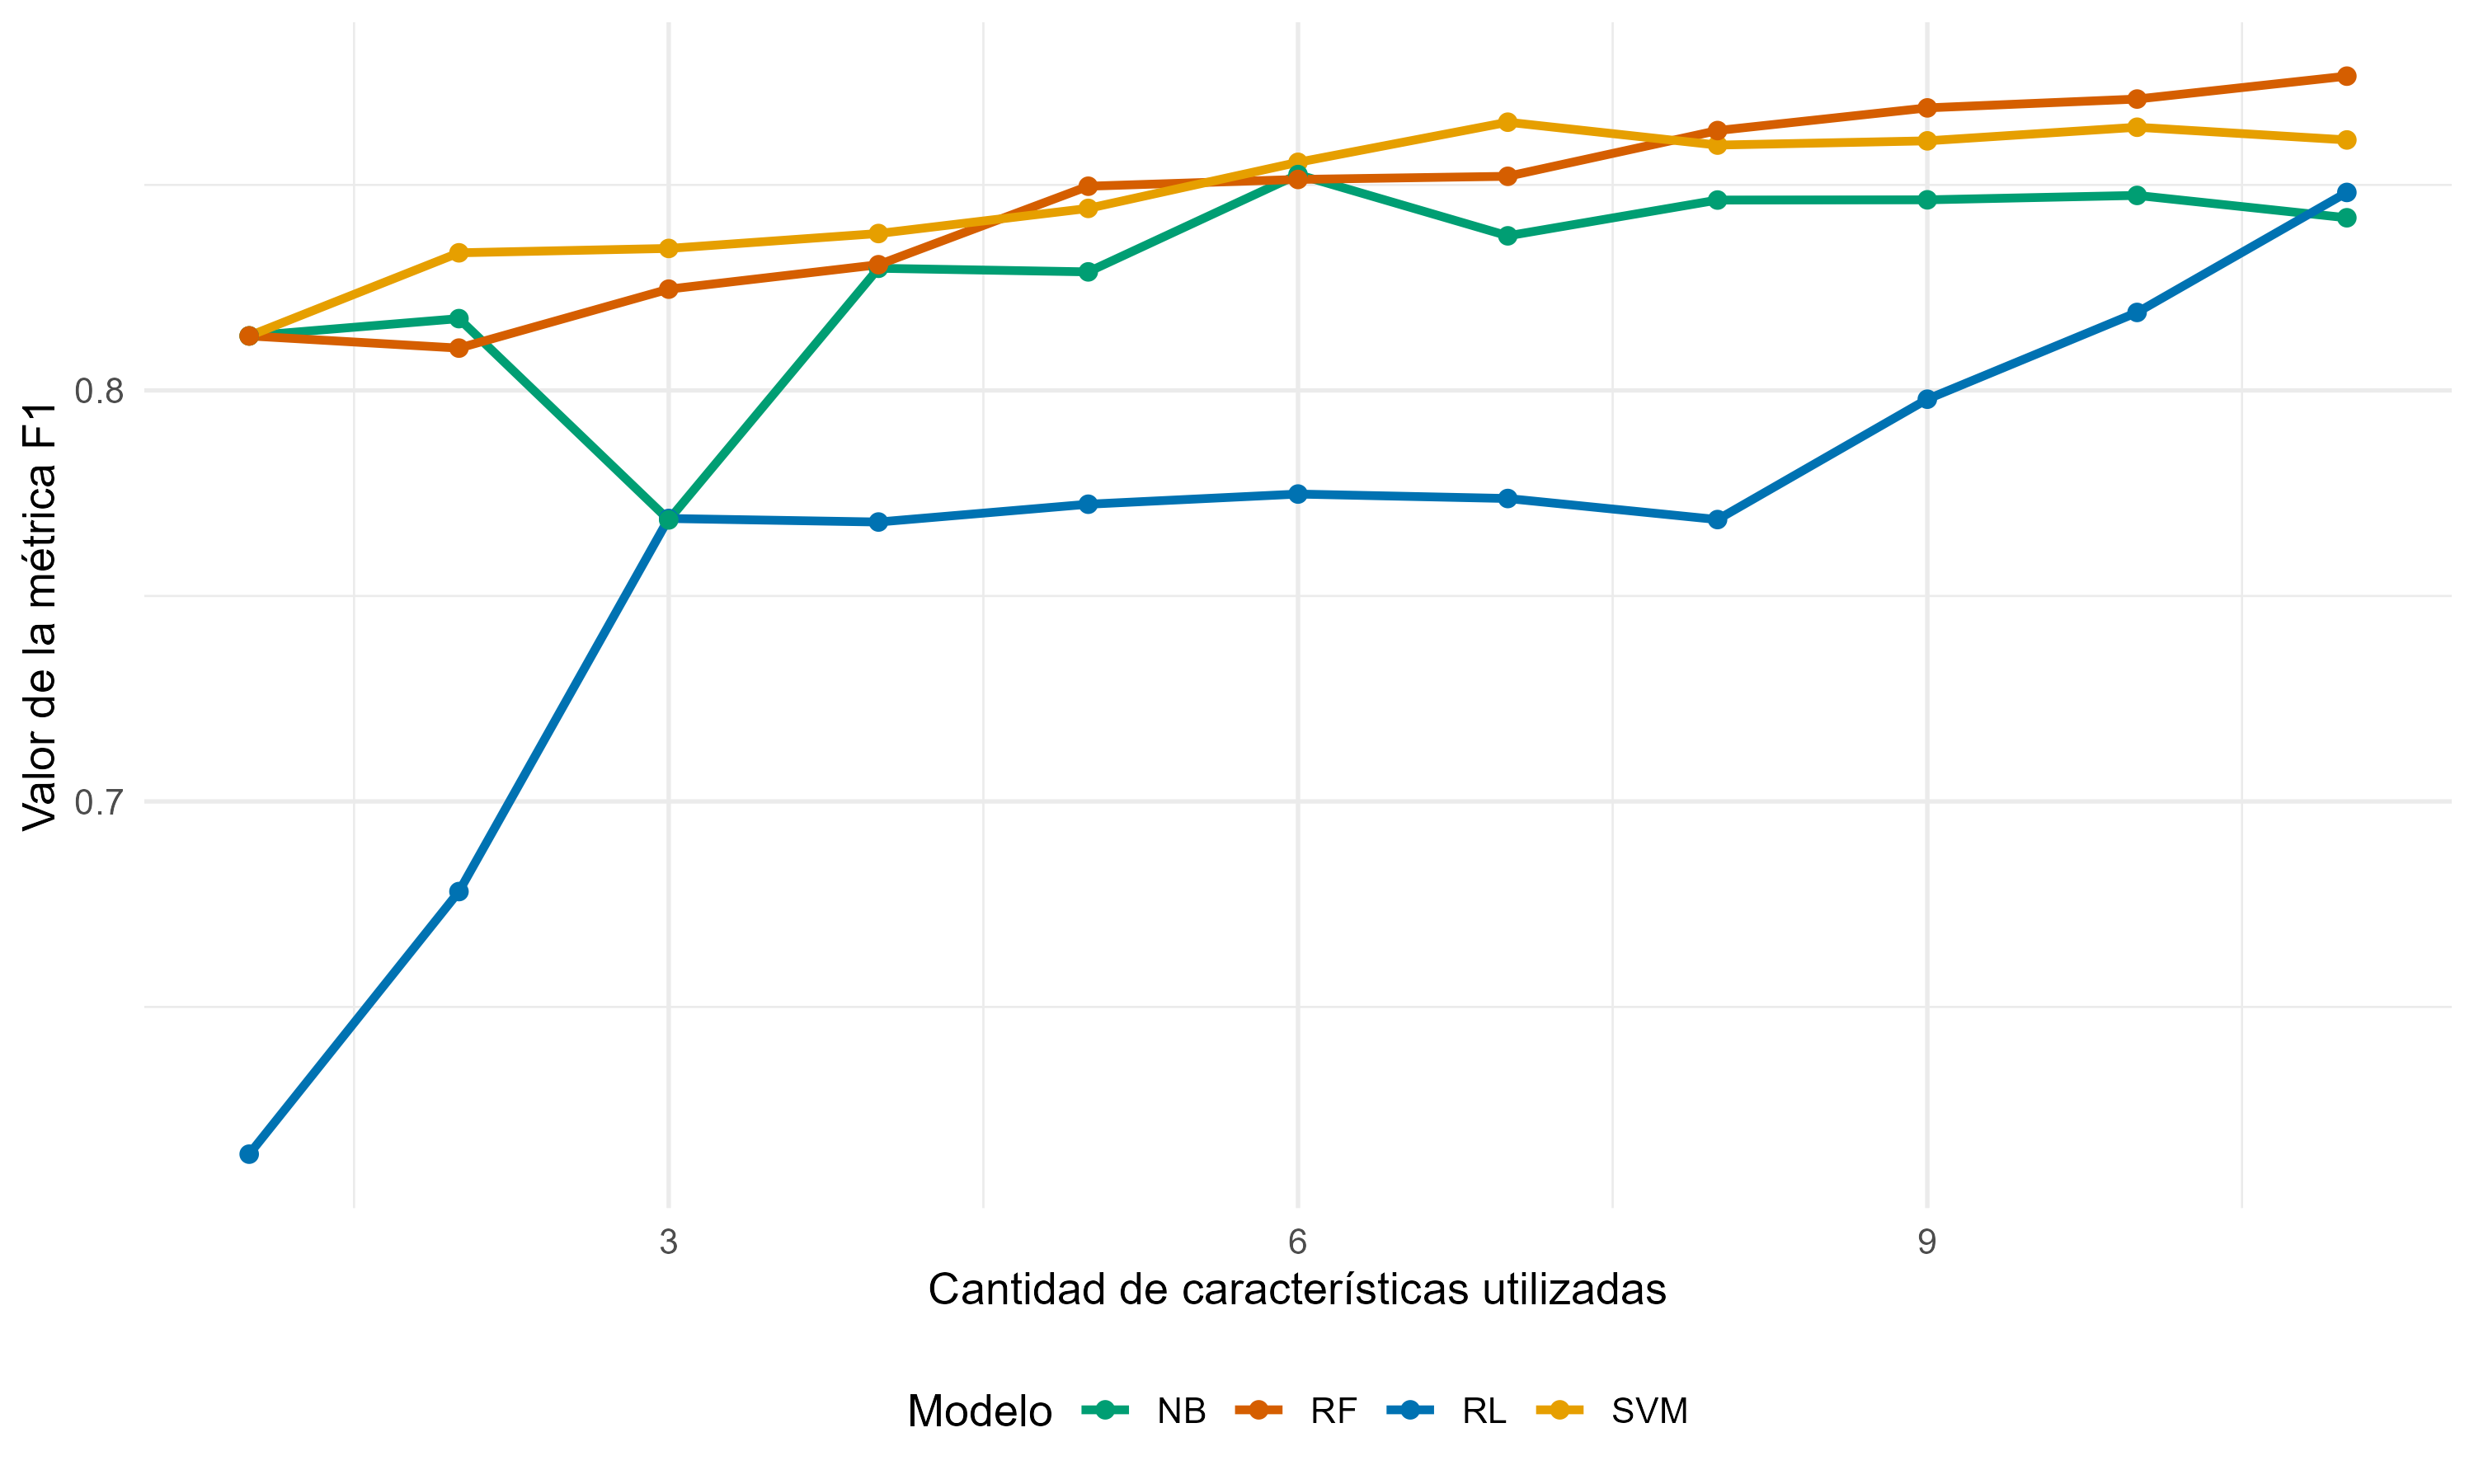
\includegraphics[width=0.49\textwidth]{evolucion_metrica_binario_F1.png}
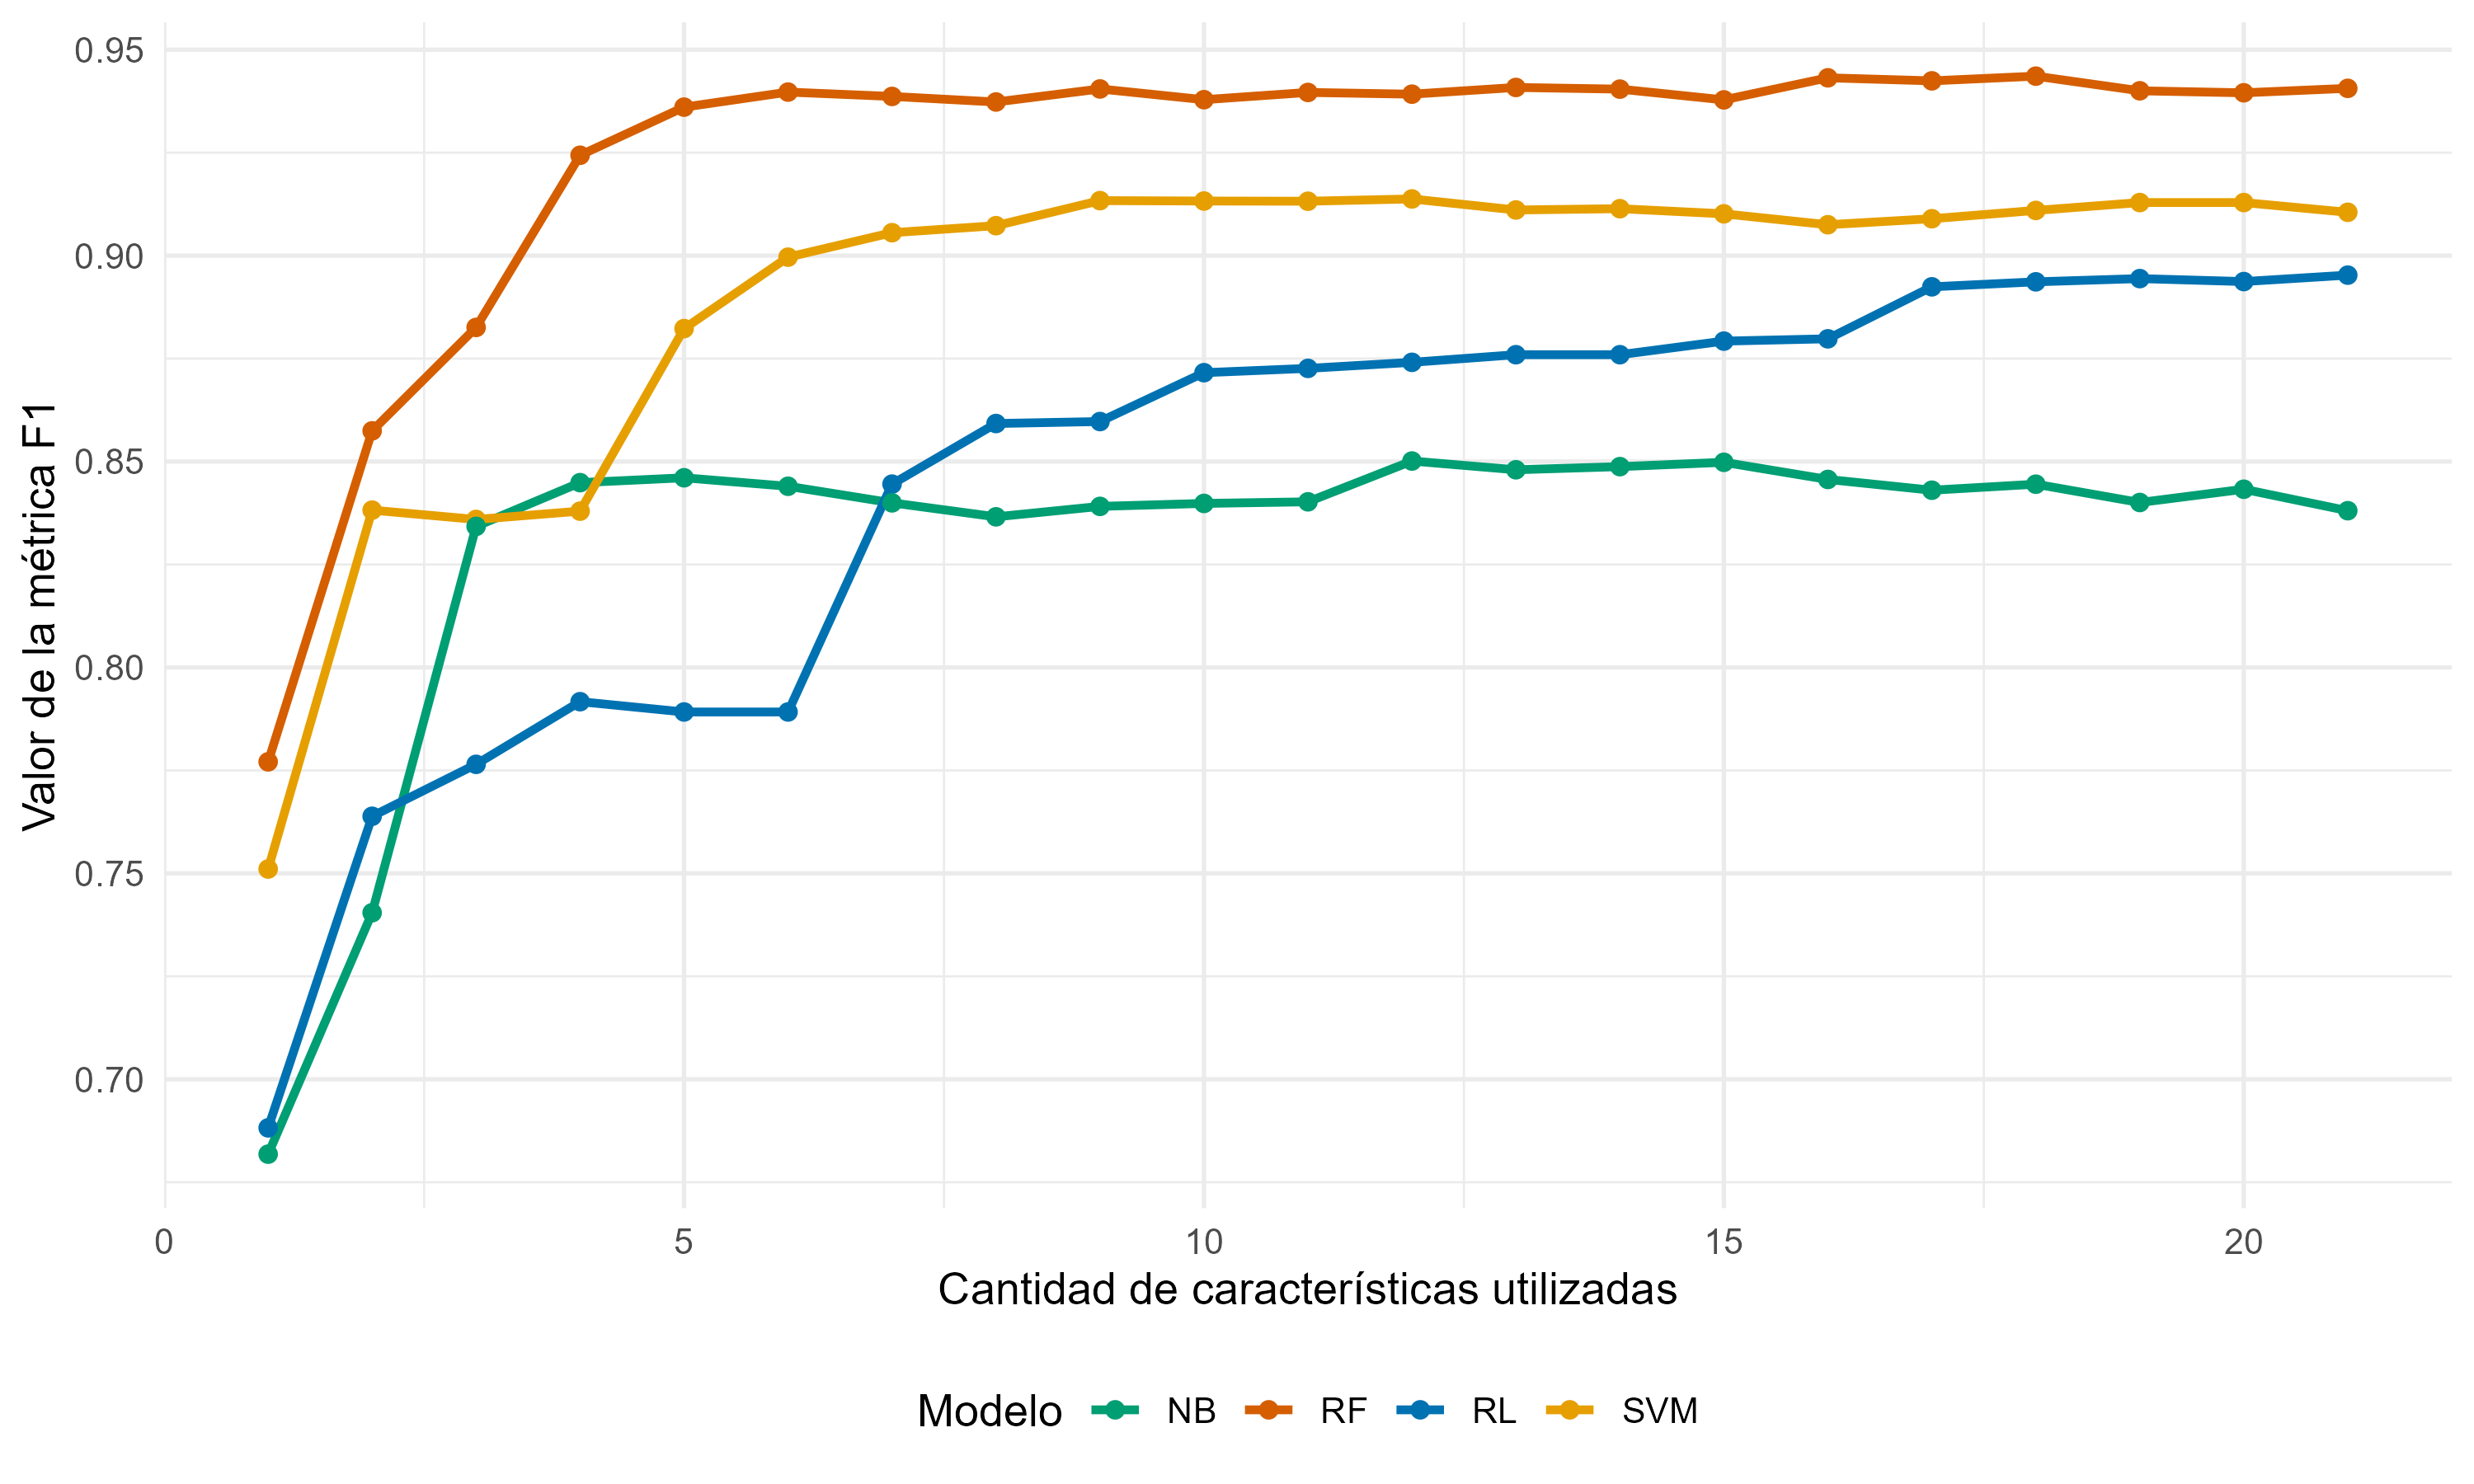
\includegraphics[width=0.49\textwidth]{evolucion_metrica_multiclase_F1.png}
\caption{Importancia de variables para los casos binario (izq.) y  multiclase (der.).} \label{fig:importancia}
\end{figure}
 
El análisis de importancia por permutación permitió evaluar cuánto influye cada variable en el desempeño del modelo adoptado. Como se observa en la Fig.~\ref{fig:importancia}, el F1-\emph{Score} aumenta en la medida en que se incorporan los atributos en orden decreciente de importancia, lo que indica que las variables mejor posicionadas aportan la mayor capacidad predictiva. Las primeras características generan el mayor incremento en el desempeño, mientras que las restantes contribuyen con mejoras marginales, evidenciando que una parte reducida de los atributos concentra la mayor parte de la información relevante. 
El análisis de importancia por permutación permitió identificar las variables más influyentes en las predicciones, donde la pendiente del segmento ST en el ECG presentó la mayor contribución en el conjunto \emph{HeartFailure}, mientras que el porcentaje de tiempo con variabilidad anormal a corto plazo fue el atributo más relevante en la base \emph{Cardiotocography}.
		





\section{Conclusiones y trabajos futuros}

Se concluye que el modelo RF es la herramienta más robusta para el tipo de datos bajo análisis debido a su capacidad para capturar relaciones no lineales y reducir el sobreajuste mediante el voto mayoritario de los árboles que lo integran. SVM también mostró un rendimiento competitivo, especialmente con \emph{kernels} radiales y polinómicos. El estudio permitió identificar atributos críticos, como la pendiente del segmento ST en el ECG y el porcentaje de tiempo con variabilidad anormal a corto plazo, para el diagnóstico de riesgo cardíaco. Como trabajos futuros, se propone el uso de optimización bayesiana para un ajuste de hiperparámetros más fino y técnicas de reducción de dimensionalidad (por ejemplo, PCA) para simplificar los modelos sin perder precisión.

\begin{credits}
\subsubsection{\ackname} Este trabajo ha sido parcialmente financiado por el proyecto PIADT PIUNAHUR-80020240200003HU.

\subsubsection{\discintname}
Los autores declaran no tener conflictos de intereses.
\end{credits}
%
% ---- Bibliography ----
%

\printbibliography[title={Referencias}]

\end{document}